\documentclass[aspectratio=169,xcolor=dvipsnames]{beamer}

\usepackage[utf8]{inputenc}  % if you want to include UTF-8 characters in your source when not using XeLaTeX or LuaTeX; also avoids biber warnings when using accents and stuff
\RequirePackage[T1]{fontenc} % Fuller font encoding
\RequirePackage{lmodern}     % Nice vector fonts
\RequirePackage[tracking]{microtype}   % Has a subtle but definite effect; most of the features aren't supported when using XeLaTeX, so if you don't need the fancy font selection from that stick with fontenc+lmodern.

\usepackage{comment}               % To comment out chunks of text
\usepackage{suffix}                % For defining command versions with *s
\usepackage[en-US]{datetime2}      % For \DTMdate, etc.

\usepackage{outlines}              % allows usage of \1, \2, \3, \4 to represent list nesting
\usepackage{epigraph}              % For epigraphs

\usepackage{booktabs}              % For nicer-looking tables
\usepackage{makecell}              % For table heading cells and cells with line breaks
\usepackage{threeparttable}        % For tables with notes

\usepackage[
  citestyle=authoryear-icomp, % Author-year style better for bibliographies
  maxcitenames=2, % for table
  maxbibnames=99 % Avoids `et al.` in bibliography
]{biblatex} % if issues occur with utf8 inputenc, try the safeinputenc option

\addbibresource{bibliography.bib}

\newcommand{\todo}[1]{{\bfseries\color{purple}#1}} % Allowing paragraphs in todos

% Beamer setup
\graphicspath{{figures/}} % for organization

\usetheme{Hokie}
\logo{\includegraphics[width=1.5cm]{vt-logo}}

\hypersetup{pdfstartview=} % Use viewer default % fits the presentation to the window when first displayed
\AtBeginSection{%
  \begin{frame}<beamer>{Outline} % Only show these frames in beamer mode; no need to shrink with other subsections hidden
    \tableofcontents[currentsection,hideothersubsections]
  \end{frame}
}

\newcommand*\blockmath[1]{%
  \vspace*{-\baselineskip}%
  \setlength\belowdisplayshortskip{0pt}%
  \[#1\]} % sometimes want a block starting with math, but starting paragraphs with math makes extra space

%% From https://brand.vt.edu/identity/color.html
% Primary Palette (There's "Yardline White" too but that's just pure white)
\definecolor{BurntOrange}{HTML}{E87722}
\definecolor{ChicagoMaroon}{HTML}{861F41}
\definecolor{HokieStone}{HTML}{75787B}

% Secondary Palette
\definecolor{PylonPurple}{HTML}{642667}
\definecolor{SkipperSmoke}{HTML}{E5E1E6}
\definecolor{SustainableTeal}{HTML}{508590}
\definecolor{VibrantTurquoise}{HTML}{2CD5C4}
\definecolor{VirginiaSunset}{HTML}{ED8B00}
\definecolor{TriumphantYellow}{HTML}{F7EA48}

% Package for flexible glossaries; I had issues with nomencl and this will allow more centralized configuration anyway. Also supports acronyms, though I am not yet transitioning those yet.
% configuring glossaries-extra to use bib2gls and also provide accessibility support just in case you want to use it for symbols or whatever that wouldn't screen-read right; treating undefined glossary entries as warnings to match standard missing-reference stuff is automatically integrated into record because of how bib2gls works.
% important: this must come AFTER hyperref, babel, polyglossia, inputenc and fontenc!
\usepackage[record,accsupp, % accessibility support
  postdot,% full stop after description; may be better to use post-description-dot per resource entry
  nostyles,% don't load default style packages; this is the recommendation
  % load glossaries-extra-stylemods.sty and tree, bookindex, long/list for abbrevs
  stylemods={tree,bookindex,long,list}, % index(group) doesn't fail when you don't include tree but latexmk errored out due to lack of stabilization
  style=indexgroup, % default style
  prefix, % for a(n) configuration
  abbreviations,symbols,index,numbers % want these glossaries
]{glossaries-extra}

\glsxtrsetgrouptitle{element}{Elements}
\glsxtrsetgrouptitle{function}{Functions}
\glsxtrsetgrouptitle{relation}{Relations}
\glsxtrsetgrouptitle{type}{Types}
\glsxtrsetgrouptitle{variable}{Variables}

\GlsXtrLoadResources[
  src=glossaries/terms
]
\GlsXtrLoadResources[
  src=glossaries/numbers, % I actually want to sort off the labels for these so no fallback needed
  type=numbers % no need for field-aliases={value=user1} as I'm putting the numbers in the symbol field anyway
]
\GlsXtrLoadResources[
  src=glossaries/elements,
  group=element,
  type=symbols,
  symbol-sort-fallback=name, % use the name instead of label for sorting
  break-at=none % prevents non-letters being discarded when sorting
]
\GlsXtrLoadResources[
  src=glossaries/functions,
  group=function,
  type=symbols, % Not sure if functions should really be treated as symbols
  symbol-sort-fallback=name,
  break-at=none
]
\GlsXtrLoadResources[
  src=glossaries/relations,
  group=relation,
  type=symbols,
  symbol-sort-fallback=name,
  break-at=none
]
\GlsXtrLoadResources[
  src=glossaries/types,
  group=type,
  type=symbols, % I thought this was unnecessary when using @symbol but it looks like category and type are not the same thing
  symbol-sort-fallback=name,
  break-at=none,
  field-aliases={format=user1}
]
\GlsXtrLoadResources[
  src=glossaries/variables,
  group=variable,
  type=symbols, % Not sure if variables should really be treated as symbols
  symbol-sort-fallback=name,
  break-at=none
]

\setabbreviationstyle{long-short-desc} % for getting full info in (alt)tree glossary
\GlsXtrLoadResources[
  src=glossaries/abbrevs,
  type=abbreviations
]

\input{preamble/listingsetup}
\usepackage{mathtools}             % For \coloneqq
\usepackage{siunitx}               % For units, S column type, nice number formatting
\usepackage{wasysym}               % For \wasylozenge
\usepackage[epsilon]{backnaur}     % For BNF diagrams; a (more complex?) alternative is the syntax package
\usepackage{bussproofs}            % for prooftree environment

%% Math commands
\newcommand*\mathasm[1]{\text{\inlineasm{#1}}}

% Memory stuff!
\newcommand*\region[2]{[#1,#2]}
\newcommand*\readmem[2]{\ast\region{#1}{#2}}
\WithSuffix{\newcommand*}\readmem*[1]{\ast#1}
\newcommand*\readmemS[3]{#1\vdash\readmem{#2}{#3}}
\WithSuffix{\newcommand*}\readmemS*[2]{#1\vdash\readmem*{#2}}
\newcommand*\htriple[3]{\{#1\}#2\{#3\}}
\WithSuffix{\newcommand*}\htriple*[4]{\{#1\}#2\{#3{;}#4\}}
\newcommand\enclosed\sqsubseteq
\newcommand\separate\bowtie
\DeclareMathOperator{\seps}{\bigotimes}

% Bots
\newcommand{\infloop}{\bot_\mathrm{NT}}
\newcommand{\err}{\bot_\mathrm{E}}

% Symbolic execution
\DeclareMathOperator{\run}{run}
\DeclareMathOperator{\loc}{loc}

% Registers and the like
\newcommand*\var[1]{\mathit{#1}}
\newcommand\retaddr{\mathtt{ret\_addr}}

% Syntactic Control Flow
\newcommand\ind[1]{\hspace{#1}}
\newcommand*\Block[2]{\mathtt{#1\texttt{->}#2}}
\WithSuffix\newcommand\Block*[3]{#1~#2~#3}
\newcommand*\ASeq{\mathrel{\texttt{;}}}
\WithSuffix{\newcommand*}\ASeq*{\texttt{;}}
\newcommand*\AWhile{\texttt{While}}
\newcommand*\ADo{\texttt{Do}}
\newcommand*\AOd{\texttt{Od}}
\newcommand*\AIf{\texttt{If}}
\newcommand*\AThen{\texttt{Then}}
\newcommand*\AElse{\texttt{Else}}
\newcommand*\AFi{\texttt{Fi}}
\newcommand*\ABB{\texttt{Block}}
\newcommand*\ASkip{\texttt{Skip}}
\newcommand*\ACall{\texttt{Call}}
\newcommand*\ABreak{\texttt{Break}}
\newcommand*\AContinue{\texttt{Continue}}
\newcommand*\AWhileResume{\texttt{Resume}}

\DeclareMathOperator{\execblock}{\textsc{symbExec}}
\DeclareMathOperator{\usage}{preserve}

\usepackage{tikz}
\usepackage{pgfplots}               % For plots

\pgfplotsset{compat=1.18}          % For up-to-date features
\usetikzlibrary{pgfplots.dateplot}  % For time formatting

\usetikzlibrary{shapes}
\usetikzlibrary{graphs}            % dot-style graph shorthands (not quite as compactible as dot language, though)
\usetikzlibrary{quotes}            % needed for quoted edge labels (only in graphs?)
\usetikzlibrary{positioning}       % For relative (=of) node positioning

\tikzset{>=stealth}

\tikzstyle{ret}=[
  isosceles triangle,
  shape border rotate=90,
  isosceles triangle apex angle=75
]
\tikzstyle{landing}=[rectangle] % wanted to use inverted triangle but it just does not look good when containing text
\tikzstyle{unwind}=[dashed,red]
\tikzstyle{interproc}=[dotted] % No red, Freek doesn't think it's worth focusing on; using red for bad/unwinding instead and changing focus so unwind is dashed
\tikzstyle{bad}=[red,fill=red,text=white]
\tikzstyle{good}=[green,fill=green,text=black]

\title[Memory Usage and Control Flow Recovery]{Low-Level Static Analysis for Memory Usage and Control Flow Recovery}
\subtitle{PhD Defense Presentation}
\author{Joshua Alexander Bockenek}
\institute[SSRG]{\includegraphics[width=2cm]{ssrg-logo}\\Virginia Tech} % Dr. Ravindran didn't like the full VT title
\subject{Static Binary Analysis}
\keywords{%
  Formal Verification,
  x86-64 Assembly,
  Interactive Theorem Proving,
  Static Binary Analysis,
  Memory Usage,
  Control Flow Recovery,
  Exception Handling%
}
\date{\DTMdate{2023-02-03}}


\begin{document}
  \frame\titlepage

  \section{Introduction}

\subsection{Motivation and Challenges}
\begin{frame}{Why static binary analysis?}
  \begin{outline}
    \1 Avoids \alert{runtime overhead}
    \2 A necessity for dynamic instrumentation
    \1 Supports symbolic, \alert{overapproximative} efforts
    \2 Vs.\ dynamic analysis being path-limited by specific inputs
    \1 Allows analysis without source code
    \2 Legacy programs
    \2 Reverse engineering
    \2 Removal of compiler from the \gls{tcb} (eliminating the \alert{semantic gap})
  \end{outline}

  \todo{rotatebox with listing in the bottom right}
\end{frame}

\frame{one more slide here would be nice}

\subsection{The Old: Preliminary Exam Recap}
\begin{frame}{What is memory usage?}
  \todo{that horizontal graph}
\end{frame}

\begin{comment} % Leaving out for now
  % \alert doesn't look good with the title bar, not enough contrast
  \begin{frame}{Memory Usage is an \emph{Overapproximation}}
    \centering
    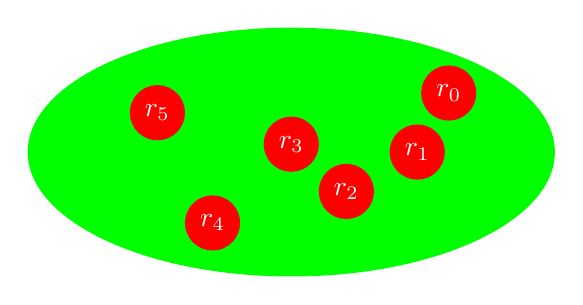
\begin{tikzpicture}[region/.style={circle, fill=red, text=white}]
      \node[ellipse, fill=green, text width=4.5cm, text height=2cm] {};
      \node[region] at (2, .75) {$r_0$};
      \node[region] at (1.6, 0) {$r_1$};
      \node[region] at (0.7, -0.5) {$r_2$};
      \node<-3>[region] at (0, 0.1) {$r_3$};
      \node<-2>[region] at (-1, -0.9) {$r_4$};
      \node<1>[region] at (-1.7, 0.5) {$r_5$};
    \end{tikzpicture}
    \vfill
    \begin{tabular}{rr}
      \textcolor{blue}{Green} & proof of no change \\
      \textcolor{blue}{Red} & no proof of no change
    \end{tabular}
  \end{frame}
\end{comment}

\begin{frame}{Floyd-Style Verification}
  \begin{columns}
    \column{.45\textwidth}
    \begin{block}{Recap}
      \begin{outline}
        \1 Approach using \glspl{cfg} deconstructed with generated \alert{cutpoints}
        \1 Generated proofs loaded in \gls{isabelle}[/HOL] and finished there
        \1 Used to verify several manually-isolated functions from \alert{the HermitCore unikernel}
        \1 Drawback: Manually intensive, proofs often require user input
      \end{outline}
    \end{block}

    \column{.45\textwidth}
    \begin{example}[Sample Graph]
    \end{example}
  \end{columns}
\end{frame}

\begin{frame}{Hoare-Style Verification}
  \begin{columns}
    \column{.45\textwidth}
    \begin{block}{Recap}
      \begin{outline}
        \1 Approach using \gls{scf} deconstructed by \alert{Hoare rules}
        \1 Generated proofs loaded in \gls{isabelle}[/HOL] and finished there
        \2 Much less interaction required, only for loops and subcalls
        \1 Used to verify dozens of HermitCore functions, including ones with subcalls; no need for manual extraction
        \1 Drawback: \gls{scf} explosion can result from spaghetti code
      \end{outline}
    \end{block}

    \column{.45\textwidth}
    \begin{example}[Sample \Gls{scf}]
    \end{example}
  \end{columns}
\end{frame}

\begin{frame}{Notice something?}
  \begin{center}
    They both rely on some form of \gls{cfr}!
  \end{center}
\end{frame}

\subsection{The New: Control Flow Recovery}
\begin{frame}{More on \Glsxtrshort{cfr}}
  \begin{outline}
    \1 Facilitates
      \2 Decompilation
      \2 Verification
      \2 Patching
    \1 Allows for improved security analyses
      \2 Can't reason over security properties if you don't know all instructions a program will go to
  \end{outline}
  \todo{put a little figure to look nice}
\end{frame}

  \section{New Related Work}

\subsection{Control Flow Recovery}

\subsection{Exception Handling Analysis}

  \section{Formally Verified Disassembly}
\begin{frame}{Breakdown of Contribution}
  \begin{outline}[enumerate] % Don't think this environment works with <+-> directly
    \1<+-> \alert{Formal models} for
      \2 State predicates
      \2 Memory relations
    \1<+-> \alert{Sound algorithm} to lift \glsxtrfullpl{hg} from binaries
    \1<+-> \alert{Evaluation} showing coverage and indirection resolution
  \end{outline}
\end{frame}

\subsection{Example}

\begin{frame}[fragile]{Full Example}{A \emph{Hoare Graph}}
  \begin{columns}
    \column{.48\textwidth}
    \begin{block}{32-bit \gls{x86} for display purposes}
      \begin{lstlisting}[style=x64,gobble=8,basicstyle=\small\ttfamily]
        0x0 : cmp eax,c3 |\label{hg-example-cmp}|
        0x5 : ja  1c     |\label{hg-example-ja}|
        0xb : mov eax,DWORD PTR [eax*4+a]|\label{hg-example-jump-table-read}|
        0x12: mov DWORD PTR [edi],eax |\label{hg-example-mov1}|
        0x14: mov DWORD PTR [esi],1   |\label{hg-example-mov2}|
        0x1a: jmp DWORD PTR [edi]     |\label{hg-example-indirect-jump}|
      \end{lstlisting}
    \end{block}

    \column{.52\textwidth}
    % combination insser sep/minimum size ensures all nodes have exactly same size
    \tikzset{vertex/.style = {circle,draw,minimum size=0.5cm}} % inner sep=0pt, <- what does this even do?
    \begin{tikzpicture}[font=\footnotesize] % if time permits play around with setting -> here
      \node[vertex]                   (0)     {$\mathtt{0}$};
      \node[vertex,right=.5cm of 0]        (5)     {$\mathtt{5}$};
      \node[vertex,above right=.1cm and .5cm of 5]  (1c)    {$\mathtt{1c}$};
      \node[draw=none,right=2cm of 1c]    (1cret) {};
      \node[vertex,below right=.1cm and .5cm of 5]  (b)     {$\mathtt{b}$};
      \node[vertex,below=.2cm of b]        (122)   {$\mathtt{12}$};
      \node[draw=none,below left=.5cm of b]    (121)   {};
      \node[draw=none,left=.1cm of 121]    (120)   {};
      \node[draw=none,below right=.5cm of b]   (123)   {};
      \node[draw=none,right=.1cm of 123]   (124)   {};
      \node[vertex,below=.2cm of 122]      (14)    {$\mathtt{14}$};
      \node[vertex,below right=.5cm of 14] (1a2)   {$\mathtt{1a}$};
      \node[vertex,below=.2cm of 1a2]      (ptr)   {$a_\mathtt{jt}$};
      \node[draw=none,right=of ptr]   (ptret) {};
      \node[vertex,below left=.5cm of 14]  (1a1)   {$\mathtt{1a}$};
      \node[vertex,below=.2cm of 1a1]      (1)     {$\mathtt{1}$};
      \node[vertex,left=of 1]         (ret)   {$a_\mathtt{r}$};

      % right tells tikz to start drawing the node right of the position (instead of centered)
      \node[right,text width=3cm,align=left] at (-1.8,.6) {\begin{align*}
          P_0 &= \readmem{\reg{rsp}}4 == a_\mathtt{r}\\
          M_0 &= \varnothing
      \end{align*}};

      \node[right=.1cm of b] {$
        \reg{eax} < \mathtt{0xc3}
        $};

      \node[right=.1cm of 122] {$
        \reg{eax} == a_\mathtt{jt}
        $};

      \node[right=.01cm of 14] {$
        \readmem{\reg{edi}}4 == a_\mathtt{jt}
        $};

      \node[right=.01cm of 1a2] {$
        \begin{array}{c}
          \gls{separate} \\
          \cdots a_\mathtt{jt}
        \end{array}
        $};

      \node[left=.1cm of 1a1] {$
        \begin{array}{c}
          \gls{alias} \\
          \cdots1
        \end{array}
        $};

      \draw [overlay,decorate,decoration={brace,amplitude=10pt,mirror},xshift=-4pt] (4.5,-1.2) -- (4.5,-.5) node [black,midway,xshift=1cm] {
        \begin{tabular}{l}
          up to\\$\mathtt{0xc3}$\\
          edges:\\one\\
          per\\read\\
          value
        \end{tabular}
      };

      \path[->] (0) edge node [above] {\inlineasm{cmp}} (5);
      \path[->] (5) edge node [above] {\inlineasm{ja}} (1c);
      \path[->] (5) edge node [below] {\inlineasm{ja}} (b);
      \draw[dotted,thick,->] (1c) edge node [above] {$\reg{eax} \geq \mathtt{0xc3}$} (1cret);
      \draw[dotted,thick,->] (b)   to (120);
      \draw[dotted,thick,->] (b)   to (121);
      \draw[->]        (b)   to (122);
      \draw[dotted,thick,->] (b)   to (123);
      \path[dotted,thick,->] (b)   edge node [right,xshift=0.2] {\inlineasm{mov}} (124);
      \path[->]        (122) edge node [right] {\inlineasm{mov}} (14);
      \path[->]        (1a2) edge node [right] {\inlineasm{jmp}} (ptr);
      \draw[dotted,thick,->] (ptr) to (ptret);
      \path[->]        (14)  edge node [left]  {\inlineasm{mov}} (1a1);
      \path[->]        (14)  edge node [right] {\inlineasm{mov}} (1a2);
      \path[line width=2pt,->] (1a1) edge node [left] {\inlineasm{jmp}} (1);
      \path[line width=2pt,->] (1) edge node [below] {{\textbf{\inlineasm{ret}}}} (ret);
    \end{tikzpicture}
  \end{columns}
\end{frame}

\begin{frame}{State of the Art}
  \begin{block}{Jakstab}
    \begin{outline}
      \1 Uses \alert{abstract interpretation}
      \1 Requires significant \alert{test harnesses}
      \1 Does not achieve full \alert{overapproximation}
    \end{outline}
  \end{block}
\end{frame}


\subsection{Formulation}

\begin{frame}{Base Algorithm}
  \begin{outline}[enumerate]
    \1<+-> Pop state off \gls{bag} of states to analyze
    \1<+-> If state \alert{``less than''} existing state in \gls{hg}, join and update \gls{hg}
    \1<+-> Evaluate current instruction in potentially-joined state; may result in multiple result states
    \1<+-> Can continue? For each result:
      \2 If yes, add to bag
      \2 If no, annotate in \gls{hg}
  \end{outline}
\end{frame}

\begin{frame}{Extension for Function Calls}
  \begin{block}{State Predicate Modifications}
    \begin{outline}
      \1<+-> External calls preserve only stack, \alert{caller-saved} registers
      \1<+-> Internal calls
        \2 Preserve stack, \alert{caller-saved} registers at call site
        \2 State within call reset, allowing reuse of results
        \2 Perform join of state-within-call and post-call state for subcall return
      \1<+-> Requires concept of \alert{reachability}; post-call states not continued unless known reachable
    \end{outline}
  \end{block}
\end{frame}

% Leaving out validation as that was Freek's work. I'll answer questions if it gets brought up but dedicating time to it explicitly is probably not worth it.

\subsection{Evaluation}

\begin{frame}{Case Study: Xen Project}
  \begin{columns}
    \column{.35\textwidth}
    \begin{center}
      \colorbox{black}{\includegraphics[width=.8\linewidth]{logo_xenproject}}\\[1em]
      \includegraphics[width=.5\linewidth]{aws_logo-100781597-large.3x2}
    \end{center}

    \column{.6\textwidth}
    \begin{block}{Properties}
      \begin{outline}
        \1 Widely used \gls{vmm}/hypervisor (e.g., Amazon AWS)
        \1 Mostly written in \gls{c}
      \end{outline}
    \end{block}
  \end{columns}
\end{frame}

% Fragile was needed with the newcolumn being inside the frame but moving it out fixed that
% number glossaries with \glsentrysymbol to get unformatted numbers weren't working so just putting the numbers directly
\begin{frame}[label=hg-results]{Statistics Summarized}
  \centering
  \begin{tabular}{l
      S[table-format=4]@{$=$}
      S[table-format=4]@{$+$}
      S[table-format=2]@{$+$}
      S[table-format=2]@{$+$}
      S[table-format=1]
      S[table-format=6]
      S[table-format=6]
      S[table-format=2]
      S[table-format=3]
      S[table-format=3]
      r}
    \toprule
    \thead{Binary Target Type} & {\thead{Total}} & {\thead{$w$}} & {\thead{$x$}} & {\thead{$y$}} & {\thead{$z$}} & {\thead{Instrs.}} & {\thead{Symbolic\\States}} & {\thead{A}} & {\thead{B}} & {\thead{C}} & \thead{Time/\\h:m:s} \\
    \midrule
    Programs & 63 & 316 & 3 & 13 & 1 & 18124 & 18562 & 56 & 26 & 11 & 0:35:59 \\
    Library Functions & 2151 & 2115 & 32 & 0 & 4 & 381647 & 391524 & 1 & 244 & 720 & 17:35:42 \\
    \bottomrule
  \end{tabular}\\
  \begin{tabular}{rcl rcl rcl}
    \multicolumn{9}{c}{$w$ lifted, $x$ unprovable return address, $y$ concurrency, $z$ timeout} \\
    A &=& Resolved indirection & B &=& Unresolved jump(s) & C &=& Unresolved call(s) \\
  \end{tabular}
  \hyperlink{timing}{\beamerskipbutton{Timing}}
\end{frame}

\begin{frame}{Discussion and Limitations}
  \begin{columns}
    \column{.35\textwidth}
    \begin{block}{Uses}
      \begin{outline}
        \1 Security analyses
        \1 Verification/\gls{tcb} reduction
        \1 Decompilation
        \1 Patching
      \end{outline}
    \end{block}

    \pause
    \column{.52\textwidth}
    \begin{block}{Limitations}
      \begin{outline}
        \1 Contextuality for return addresses, indirection
        \1 No concurrency support
        \1 No \gls{cpp} \gls{eh} support
          \2 Not an issue for Xen, but\dots
      \end{outline}
    \end{block}
  \end{columns}
\end{frame}

  \section{Exceptional Interprocedural Control Flow Graphs}

\subsection{Example}
\frame{dummy}
\begin{frame}{Ghidra-Generated Example}
  \centering
  % Trying to use \only/\uncover/etc. with the graph paths directly doesn't work so need to mess with the styles
  \only<1>{
    \tikzstyle{unwind}=[draw=none]
    \tikzstyle{interproc}=[draw=none]
    \tikzstyle{bad}=[]
    \tikzstyle{good}=[]
  }
  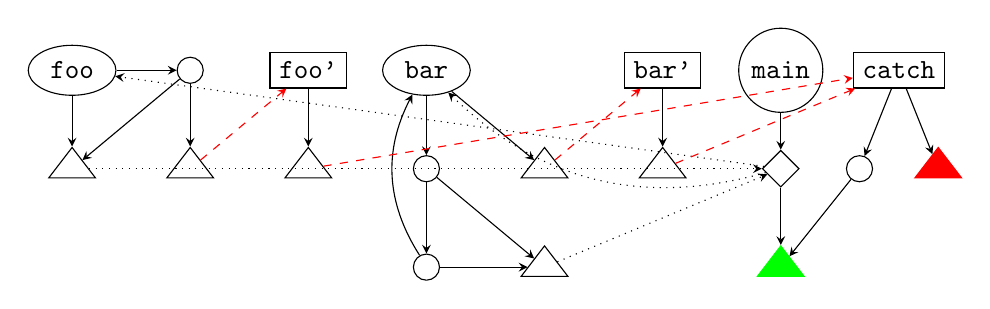
\begin{tikzpicture}
    \graph[
      grow down=1.25cm,
      branch right=1.5cm,
      nodes={draw,ellipse,font=\ttfamily}
    ]{
      foo -> fEnd1/""[ret],
      foo -> "" -> {fEnd1, fEnd2/""[ret]}, % more compact this way
      foo'[landing] -> fEnd'/""[ret],

      bar -> {b1/"", bEnd1/""[ret,< draw=none]} -> {b2/"", bEnd2/""[ret]},
      b2 -> {bar[> bend left], bEnd2},
      b1 -> bEnd2, % necessary due to group/chain interactions
      bar'[landing] -> bEnd'/""[ret],

      {[grow down=1.25cm, branch right=1.5cm]
        {main[circle], catch[landing]} -> {
          callSite/""[diamond],
          ""[at=(0:-.5)],
          ""[ret, bad, at=(0:-1), < draw=none]
        } -> ""[ret,good],
      };

      callSite ->[interproc] foo;
      callSite ->[interproc] bar;

      fEnd1 ->[interproc] callSite;
      bEnd2 ->[interproc] callSite;

      fEnd2 ->[unwind] foo'; fEnd' ->[unwind] catch;
      bEnd1[< draw] ->[unwind] bar'; bEnd' ->[unwind] catch; % Had to reenable bEnd1's ability to draw outgoing edges here as setting it on the edge itself didn't work.
    };
  \end{tikzpicture}
  \uncover<2->{
      \begin{description}[leftmargin=\widthof{Green triangle}]
      \item[Red dashes] normal interprocedural control flow
      \item[Blue dots] unwinding edges
      \item[Green triangle] successful termination
      \item[Blue triangle] exceptional termination
    \end{description}
  }
\end{frame}

\subsection{Formulation}
\frame{dummy}

\subsection{Validation}
\frame{dummy}

\subsection{Results}
\frame{dummy}

\subsection{Discussion}
\frame{dummy}

  \section{Future Work}

\subsection{Contextuality}
\frame{dummy}

\subsection{Concurrency}
\frame{dummy}

\subsection{State Space Reduction}
\frame{dummy}

% TODO: Why do the gls fmt commands not work in beamer sectioning?
\subsection{Integrating \Glsfmtshort{cfr} into Formal Frameworks}
\frame{dummy}


  \appendix % Not sure if this is really right but oh well
  \begin{frame}%[t,allowframebreaks]
    \frametitle{Bibliography}
    \printbibliography[heading=none] % sections in frames is a no-no
  \end{frame}
\end{document}
